\chapter{Hydrodynamics of Vegetated Lateral Cavities}
\label{chap:art2}
In this chapter, the second topic of the dissertation is presented as a published conference paper. This paper was originally written in Portuguese and was translated for this dissertation. The objective of this paper was to develop a simple numerical method capable of estimating the flow and the mass exchange between a lateral cavity and the main channel. 

The original paper was published in the '17º Congresso Nacional do Meio Ambiente', on September 24th 2020, Poços de Caldas, Brazil.
\section*{Authors}
\begin{itemize}
    \item Luiz Eduardo Domingos de Oliveira \footnote{Federal University of Mato Grosso do Sul}
    \item Taís Natsumi Yamasaki \footnotemark[1]
    \item Felipe Rezende da Costa \footnotemark[1]
    \item Johannes Gérson Janzen \footnotemark[1]
    \item Carlo Gualtieri \footnote{University of Naples Federico II}
\end{itemize}
\addcontentsline{toc}{section}{Abstract}
\section*{Abstract}
In rivers and channels, dead zones are regions of low velocity with the presence of recirculation motion, that have important ecological functions (eg. sediment retention) and also can be formed from human-made structures (eg. transversal dikes). The presence of vegetation in dead zones is a new topic of this discussion opening its way in the vegetated flow area of study, as the vegetation has the potential of changing the flow and altering mass exchange processes with the main channel. This study aimed to develop a numerical model of a single vegetated lateral cavity using Computational Fluid Dynamics (CFD). The vegetation drag was represented by a porous media which coefficients were calculated from experimental data. The results of the model shown that the cavity had a single vortex system in its interior and the flow velocity varied from $-0.11$ to $ 0.24 cm/s$. The simulation adapted well to the experimental data, which proved that the porous media is a suitable method of representing the vegetation drag in CFD.

\noindent\textbf{Keywords:} Lateral Cavities; Vegetation; Computational Fluid Dynamics (CFD).

\section{Introduction}
Rivers are formed by complex morphological boundaries, that create a variety of regions of high or low flows. One of these regions is named dead zone, in which slow velocities occur when compared to the main channel. The dead zones can occur naturally through lateral cavities \cite{jackson2013} or in man-made structures, groyne fields \cite{sukhodolov2017} and transversal dikes \cite{Pandey2018}. From the environmental point of view, dead zones function a 'foam' that absorbs part of the energy from the flow, which causes it to favour the retention of sediments, the protection of the margins and creates a habitat for biota that depends on slow waters \cite{Weitbrecht2008}.

In the field of vegetated flows, in which the main objective is to study the hydrodynamics between the flow and the vegetation, the research of vegetated dead zones is still recent. The presence of vegetation in the dead zone offers an additional drag to the flow, further impacting the velocity patterns in the region. Henceforth, the mass exchange processes between the main channel and the dead zone are also altered \cite{xiang2019}. This enlightens the importance of understanding the relationships, so it could be better used aiming to benefit the surrounding ecosystem. This study aims to simulate through Computational Fluid Dynamics (CFD) a vegetated lateral cavity using a porous media to represent the vegetation.

\section{Methods}
The chosen geometry consisted of a part of a channel and a lateral cavity (Figure \ref{fig:art2:compDomain}) based in \cite{xiang2019}. The depth of the flow and the channel ($H$) was defined in $0.10\,m$ and the channel width ($B$) in $0.30\,m$. The cavity was $L=0.25\,m$ long and $W=0.15\,m$ wide. The mean velocity was kept constant as $U=0.101\,m/s$, which corresponded to a Reynolds number of $Re=9000$ (turbulent flow). The water was kept at a constant temperature of $T=293$ K.

\begin{figure}[!ht]
\centering
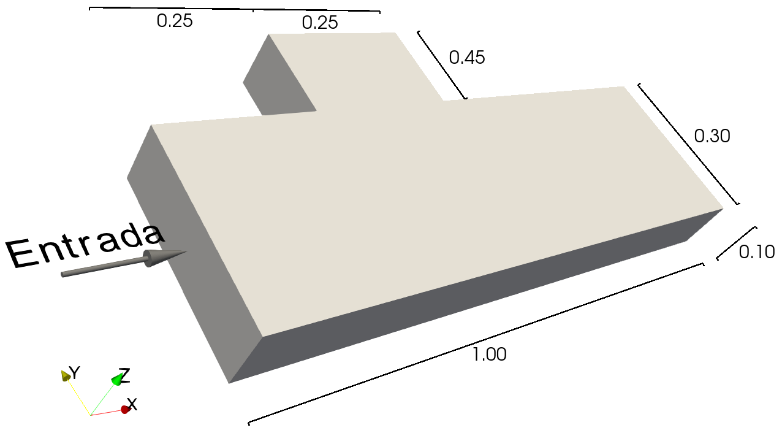
\includegraphics[width=\linewidth]{../images/art2/imgHyd1.png}
\caption{Computational domain. The flow direction is indicated by the grey arrow ('Entrada'). The dimensions are in metres and the coordinate origin ($x, y, z = 0$) at the lower right portion of the channel.}
\label{fig:art2:compDomain}
\end{figure}
The used boundary conditions were a longitudinal plane that cuts the domain at $y=0$ and at the top of the domain ($z=0.10$ m) that were defined as slip surfaces. The planes that cut the left portion of the channel and the cavity walls were considered hydraulic smooth walls of zero velocity. The channel entrance ($x=0\,m$) imported a velocity profile previously simulated in a periodic channel. The outlet surface ($x=1.00\,m$) was calculated with a zero gradient function.

The vegetation was represented with a porous media that filled all the lateral cavity. This is a simple way to represent the vegetation drag, and yet being an effective method of capturing the hydrodynamic effects \cite{Yamasaki2019}.  The adopted porous media was calculated by the Darcy-Forchheimer model (DF), that divides the drag into viscous and inertial resistances. The coefficients were calculated using the Ergun formulation and \textcite{Sonnenwald2017}, the vegetation parameters used to calculate the coefficients for the DF were taken from the second case of \textcite{xiang2019}. The details of the used methods can be found in the user's guide of \textit{Fluent}\textsuperscript{\textregistered}.

The numerical model was simulated under the commercial software \textit{Fluent}\textsuperscript{\textregistered} (version 14), using the method of finite volumes to discretise the governing equations of mass conservation and momentum. The turbulence model applied was the Detached Eddy Simulation, with the contour model using the k-omega Shear Stress Transport. The simulation ran under a transient configuration for 350 seconds, that was enough time to stabilise the flow.
\section{Results and Discussion}
As expected, the flow inside the cavity became slower when compared to the main channel, the x component of the velocity varied between $0.11$ and $0.25U$ (Figure \ref{fig:art2:velCont}). The high-velocity gradient in the cavity entrance ($y=0.30\,m$) formed a shear layer that originated the vortexes. These vortexes were carried inside the cavity where a single circulation system, concentrated to the right portion, occurred as the streamlines in Figure \ref{fig:art2:velCont} indicates. The adjusted drag coefficients were: $83.37\,m^2$ for the viscous resistance and $3.79\,m^{-1}$ for the inertial resistance.

\begin{figure}[!ht]
\centering
\begin{subfigure}{0.49\textwidth}
  \centering
  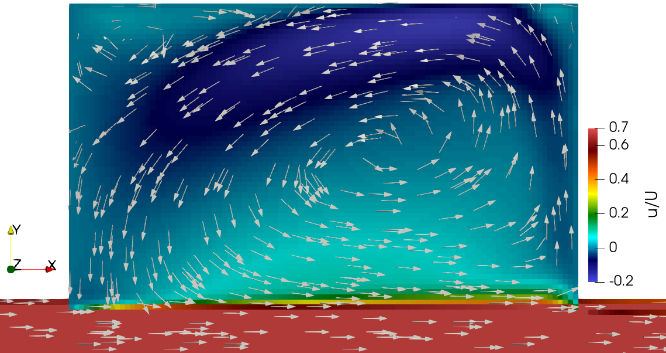
\includegraphics[width=0.9\linewidth]{../images/art2/imgHyd2.png}
  \caption[width=0.9\linewidth]{Contour and streamlines of the mean x-velocity.}
  \label{fig:art2:velCont}
\end{subfigure}%
\begin{subfigure}{.49\textwidth}
  \centering
  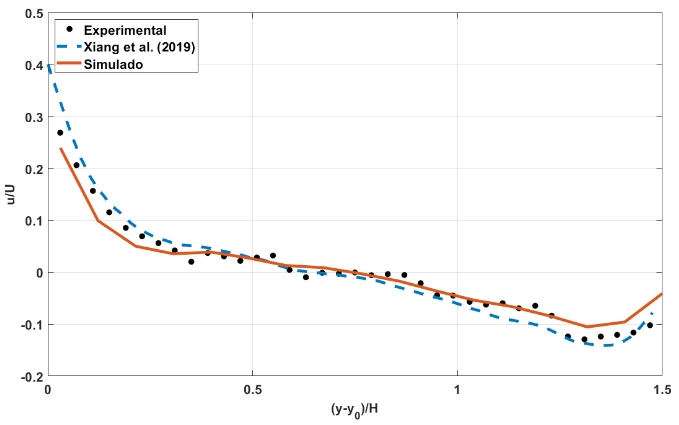
\includegraphics[width=0.9\linewidth]{../images/art2/imgHyd3.png}
  \caption[width=0.9\linewidth]{Mean velocity profile considering only the region inside the cavity.}
  \label{fig:art2:velProf}
\end{subfigure}
\caption{Velocity distributions along the plane $z=0.60H$.}
\label{fig:art2:velz06H}
\end{figure}
The y-velocity data was extracted along the plane $z=0.6H$ and condensed in a line using an ensemble averaging procedure along the y-axis similar to the procedure adopted in \textcite{sukhodolov2014}. The velocity profile is shown and compared with numerical and experimental data extracted from the literature in the Figure \ref{fig:art2:velProf}. At the entrance of the cavity ($(y-y_0)/H = 0$), the velocity $u$ was $0.25U$ and it kept getting slower as it moved towards the interior of the cavity. In $(y-y_0)/H = 1.4$, the flow got a negative value of $u = -0.1U$, indicating the presence of vortexes. The presented model, in orange, was well adjusted to the experimental data (black dots). This means that the porous media coefficients were well calculated and the model was capable of reproducing the flow in a accordance to the laboratory experiments.

\section{Conclusion}
The porous media model was capable of representing the vegetation in the numerical simulation. The cavity presented a single circulation system with a slower velocity than the main channel. The velocity profile obtained from the simulation was well adjusted to the experimental data, which further demonstrates that the model was capable of capturing the effects of vegetation inside the cavity.

%\nomenclature{$H$}{Flow Depth\nomunit{$m$}}
%\nomenclature{$B$}{Experimental channel width\nomunit{$m$}}
%\nomenclature{$W$}{Lateral cavity width\nomunit{$m$}}
%\nomenclature{$L$}{Lateral cavity length\nomunit{$m$}}
%\nomenclature{$U$}{Mean streamwise velocity in the main channel\nomunit{$m/s$}}
%\nomenclature{$Re$}{Reynolds number}
%\nomenclature{$T$}{Temperature\nomunit{$K$}}
%\printnomenclature

\addcontentsline{toc}{section}{Funding}
\section*{Funding}
This study was financed in part by the Coordenação de Aperfeiçoamento de Pessoal de Nível Superior - Brazil (CAPES) -Finance Code 001.
\addcontentsline{toc}{section}{References}
\printbibliography[segment=\therefsegment,heading=subbibliography, title={References}]